\documentclass{standalone}

\usepackage[svgnames]{xcolor}
\usepackage{tikz}

\usepackage{amsmath}
\usepackage{amssymb}


\begin{document} 

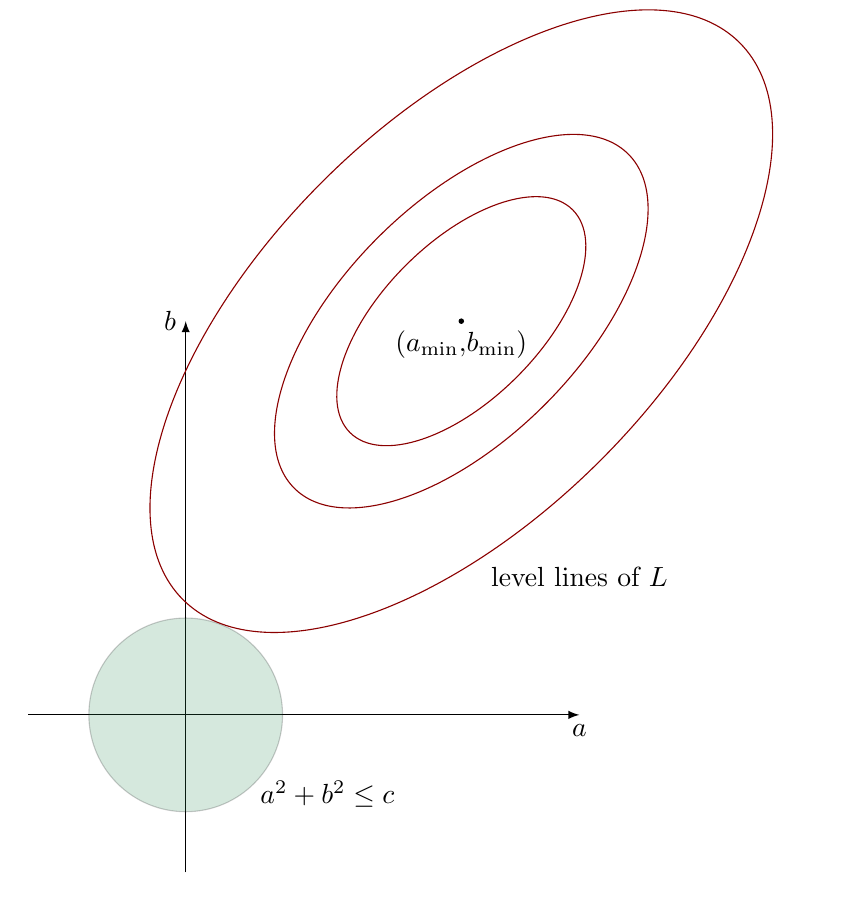
\begin{tikzpicture} 
\draw[-latex] (-2,0) -- (5,0) node[below]{$a$};
\draw[-latex] (0,-2) -- (0,5) node[left]{$b$};
\filldraw[opacity=0.2,fill=SeaGreen] (0,0) circle [radius=1.23];
\coordinate[label=below:$(a_{\text{min}}{,}b_{\text{min}})$] (beta) at (3.5,5);
\fill (beta) circle (1pt);
\foreach \X in {1,1.5,2.5}
{\draw[rotate=45,DarkRed] (beta) circle({2*\X} and {1.0*\X});}
\coordinate[text=DarkRed, label=level lines of $L$] (txtlbl) at (5,1.5);
\coordinate[text=SeaGreen, label=$a^2+b^2 \leq c$] (txtlbl2) at (1.8,-1.3);

\end{tikzpicture} 
\end{document} 